\documentclass[11pt,a4paper]{ltjsarticle}
\usepackage{luatexja-fontspec}
\usepackage{amsthm}
\usepackage{enumitem}
\usepackage{sty/mathnotation}
%\usepackage{unicode-math}
%\setmathfont{Latin Modern Math}
\usepackage{amsmath,amssymb}
\usepackage[colorlinks=true,unicode,linkbordercolor={0 0 0}]{hyperref}
\usepackage{cleveref}
\usepackage{authblk}
\usepackage{diffcoeff}
\usepackage{bigints}
\usepackage[margin=25mm,truedimen]{geometry}
\usepackage[labelsep=quad]{caption}
\usepackage{subcaption}
\usepackage{graphicx}
%
%
%
%
\setfraction
%
%
\newcommand*{\definition}[1]{\textbf{#1}}
\newcommand*{\length}[1]{\overline{#1}}
\newcommand*{\equivalent}{\Longleftrightarrow}
\newcommand*{\coord}[1]{\paren{#1}}
\newcommand*{\intd}{\dl2}
\newcommand*{\restrict}{\upharpoonright}
\newcommand*{\image}[2]{#1 \sqbracket*{#2}}
\newcommand*{\inv}[1]{{#1}^{-1}}
\newcommand*{\neighbourfood}[2]{\apply{N}{{#1};{#2}}}
\delimitershortfall = -0.5pt
%
%
%
\crefname{figure}{図}{図}
\crefname{equation}{式}{式}
\crefname{que}{問}{問}
\crefname{ans}{解答}{解答}
\crefname{lemma}{補題}{補題}
\crefname{dfn}{定義}{定義}

\newcommand\crefrangeconjunction{--}
\newcommand\crefpairconjunction{, }
%
%
\theoremstyle{definition}
%
%
\setlist[1]{
labelindent = \parindent,
itemindent = \parindent
}
\setlist[enumerate,1]{
  label = {(\arabic*)},
  ref = \arabic*
}
%
\newtheorem{dfn}{定義}[section]
\newtheorem{thm}[dfn]{定理}
\newtheorem{ex}[dfn]{例}
\newtheorem{que}[dfn]{問題}
\newtheorem{ans}[dfn]{解答}
\newtheorem{lemma}[dfn]{補題}
\newtheorem{coro}[dfn]{系}

%
\title{高校数学$+\alpha$でできる(実)三角関数論の精密化}
\author{野口匠}
\affil{高知工科大学大学院工学研究科}
\date{\today}

\begin{document}
%
\maketitle

\begin{abstract}
  「高校の数学Ⅲの教科書における$\lim_{x \to 0} \frac{\sin x}{x} = 1$の証明は循環論法である」
  という主張は受験業界でたびたび耳にする.そして,「循環論法を回避する方法」として,無限級数や微分方程式を用いた
  やや高度な前提知識を要するもの,あるいは高度な前提知識こそ不要であるが直感的でないため
  高校の教科書に載っている三角関数の同等の概念を扱っていることが明瞭でないもの
  が提示されることもある.本稿では,「(実数の範囲での)三角関数論は高校の教科書に載っている事項
  と積分に関する基本事項のみで厳密に展開することができ,
  かつ高校の教科書での議論の展開の仕方を大きく修正する必要はない」ということを実例でもって示す.
  なお,本稿で提示する内容は筆者オリジナルのものではなく,インターネット上に断片的に存在する情報をまとめ上げ,必要に応じて
  解説を付け加えたものである.
\end{abstract}


\section{準備} \label{sec:pre}

\subsection{記法} \label{subsec:notation}

この記事では,以下のような表記法を採用する.
なお,高校の教科書における流儀とは異なる部分が多数見られるので注意せよ.

\begin{itemize}
  \item 点を表す記号は高校の教科書ではローマン体で$\mathrm{A}, \mathrm{B}, \dotsc$のように
        書かれることが多いが,この記事では通常の変数と同じく$A,B, \dotsc$のようにイタリック体で表記する.
  \item 集合$S$と条件$\varphi$に対し,$\varphi$を満たす$S$の元全体の集合を$\setintension{x \in S}{\apply{\varphi}{x}}$と表す.
  \item 実数全体の集合を$\Real$で,(ユークリッド)平面を$\Real ^2$でそれぞれ表す.
        $x \in \Real$は$x$が実数であることを,$P \in \Real ^2$は$P$が平面上の点であることをそれぞれ表す.
  \item 「座標が$\coord{a,b}$であるような点$P$」を
        この記事では「$P = \coord{a,b}$」と表すこととする.
  \item $x < y$または$x = y$であることを表す不等号として$x \leq y$を用いる.
  \item 実数の連続性に起因する関数や広義積分の性質に関しては深入りしない.これらに関しては初等的な微分積分学の教科書を参照せよ.
  \item 集合に関する基本的な記法や性質は既知とする.
  \item 2つの集合$X,Y$に対し,$f$が$X$から$Y$への写像であることを$f \colon X \to Y$と表す.
        写像は関数を拡張した概念だと思えばよい.
  \item 集合$X, Y$に対し,$x \in X$を$y \in Y$に対応させる写像を$X \ni x \mapsto y \in Y$と表す.
        $f \colon X \to Y$は$f$が$X$から$Y$への写像であるという主張を表す記号列であったが,
        $X \ni x \mapsto y \in Y$は写像そのものを表す記号列であることに注意せよ.
  \item 集合$A,B$に対し,$A$に属するが$B$に属さない元全体の集合を$A \setminus B$と表す.
        すなわち,$A \setminus B = \setintension{x \in A}{x \notin B}$である.
  \item 写像$f \colon X \to Y$に対し,集合$\setintension{\apply{f}{x} \in Y}{x \in X}$を$\image{f}{X}$と表す.
        $f$が関数のときには$\image{f}{X}$は$f$の値域と呼ばれることが多い.
  \item 実数$a$と正の実数$\delta$に対し,開区間$\interval{op}{a - \delta, a + \delta}$を
        $a$の$\delta$近傍といい,$\neighbourfood{a}{\delta}$と表す.
\end{itemize}

\subsection{微分積分学からの準備} \label{subsec:calculus}

三角関数が曲線の長さや逆関数を用いて記述される以上,
実数の連続性に関する議論を避けることはできない.
ここでは,特に強調しておくべき性質を証明抜きで列挙する.
なお,円の対称性を利用すれば本稿から広義積分を完全に消し去ることも可能である.
しかし,そのようなことをしても無駄に手間がかかり議論の見通しが悪くなるだけなので素直に導入する.

\begin{thm} \label{thm:derivcont}
  点$a$と$a$のある$\delta$近傍$\neighbourfood{a}{\delta}$を含む$\Real$の部分集合$X$上で定義された関数$f \colon X \to \Real$が
  $\neighbourfood{a}{\delta}$上で連続で,
  $\neighbourfood{a}{\delta} \setminus \setextension{a}$上で微分可能であるとする.
  このとき,$\lim_{x \to a} \apply{f'}{x}$が
  存在するならば,$f$は点$a$で微分可能であって
  $\apply{f'}{a} = \lim_{x \to a} \apply{f'}{x}$である.
\end{thm}



\begin{thm} \label{thm:invderi}
  関数$f \colon X \to Y$は全単射で,かつ$X$上で微分可能であるとする.
  このとき,任意の$x \in X$に対して$\apply{f'}{x} \neq 0$であるならば,
  $f$の逆関数$\inv{f} \colon Y \to X$は$Y = \image{f}{X}$上の
  各点$b = \apply{f}{a}$ ($a \in X$)で微分可能であって,
  \begin{align}
    \apply{\paren{\inv{f}}'}{b} = \frac{1}{\apply{f'}{a}} \text{.}
  \end{align}
\end{thm}

\begin{thm} \label{thm:injection}
  狭義単調関数は単射である.
\end{thm}

\begin{thm} \label{thm:image}
  閉区間$\interval{c}{a,b}$上で定義された連続関数$f \colon \interval{c}{a,b} \to \Real$は
  最大値と最小値をもち,その最大値と最小値をそれぞれ$M,m$とおくと,
  $f$の値域$\image{f}{\interval{c}{a,b}}$は閉区間$\interval{c}{m,M}$である.
  すなわち,任意の$x \in \interval{c}{a,b}$に対して$m \leq \apply{f}{x} \leq M$であり,
  かつ任意の$\gamma \in \interval{c}{m,M}$に対して$\apply{f}{c} = \gamma$となる
  $c \in \interval{c}{a,b}$が存在する.
  特に,$f$の終域を閉区間$\interval{c}{m,M}$にとりかえて得られる写像
  \begin{align}
    \interval{c}{a,b} \ni x \mapsto \apply{f}{x} \in \interval{c}{m,M}
    \label{eq:surjec}
  \end{align}
  は全射である.
\end{thm}

\begin{thm}[微分積分学の基本定理] \label{thm:int}
  閉区間$\interval{c}{a,b}$上で定義された連続関数$f \colon \interval{c}{a,b} \to \Real$
  の定積分
  \begin{align}
    \int_a^b \apply{f}{x} \intd x
    \label{eq:int}
  \end{align}
  の値が(適切な定義のもとで)確定する.
  さらに,任意の$c \in \interval{c}{a,b}$に対し,関数
  \[
    \interval{c}{a,b} \ni x \mapsto \int_c^x \apply{f}{t} \intd t \in \Real
  \]
  は開区間$\interval{op}{a,b}$上で微分可能であって,各$x \in \interval{op}{a,b}$に対して
  \begin{align}
    \diff*{\int_c^x \apply{f}{t} \intd t}x = \apply{f}{x}
    \label{eq:intderi}
  \end{align}
  が成り立つ.
\end{thm}

\begin{dfn} \label{dfn:impint}
  半開区間$\interval{lop}{a,b}$上で定義された連続関数$f \colon \interval{lop}{a,b} \to \Real$について,
  極限
  \begin{align}
    \lim_{\varepsilon \to +0} \int_{a + \varepsilon}^b \apply{f}{x} \intd x
    \label{eq:impintlim}
  \end{align}
  を$f$の\definition{広義積分}といい,
  \begin{align}
    \int_a^b \apply{f}{x} \intd x
    \label{eq:impint}
  \end{align}
  と表す.\Cref{eq:impintlim}が収束する場合,その極限値をこの広義積分の値とする.
  また,$f$の定義域を半開区間$\interval{rop}{a,b}$におきかえたものに対しても同様にして広義積分を定義する.
  さらに,開区間上$\interval{op}{a,b}$上で定義された連続関数$f \colon \interval{op}{a,b} \to \Real$
  に対しては,$c \in \interval{op}{a,b}$の任意にとり,2つの広義積分
  \begin{align*}
    \int_a^c \apply{f}{x} \intd x , \int_c^b \apply{f}{b} \intd x
  \end{align*}
  がともに収束する場合,
  \begin{align}
    \int_a^b \apply{f}{x} \intd x = \int_a^c \apply{f}{x} \intd x + \int_c^b \apply{f}{x} \intd x
    \label{eq:impintop}
  \end{align}
  として$f$の広義積分の値を定義する.この値は$c$に依存しない.

  無限区間$\interval{rop}{a, \infty}$で定義された連続関数$f \colon \interval{rop}{a , +\infty} \to \Real$
  に対しては,
  極限
  \begin{align}
    \lim_{M \to \infty} \int_a^M \apply{f}{x} \intd x
    \label{eq:impliminfty}
  \end{align}
  を$f$の広義積分といい,
  \begin{align}
    \int_a^{\infty} \apply{f}{x} \intd x
    \label{eq:impintinfty}
  \end{align}
  と表す.\Cref{eq:impliminfty}が収束する場合にその極限値をこの広義積分の値とする点は同様である.
  その他の無限区間上で定義された連続関数の広義積分も上記のものと同様に定義する.
\end{dfn}

\begin{thm} \label{thm:impintconv}
  半開区間$\interval{lop}{a,b}$上で定義された連続関数$f \colon \interval{lop}{a,b} \to \Real$
  について,極限
  \begin{align}
    \lim_{x \to a+0} \paren{x - a}^p \absolute{\apply{f}{x}}
    \label{eq:limimpint}
  \end{align}
  が有限確定であるような$0 < p < 1$を満たす実数$p$が存在するならば,
  \cref{eq:impint}の広義積分は(絶対)収束する.
  また,半開区間$\interval{rop}{a,b}$上で定義された連続関数$f \colon \interval{rop}{a,b} \to \Real$
  について,極限
  \begin{align}
    \lim_{x \to b - 0} \paren{b - x}^p \absolute{\apply{f}{x}}
    \label{eq:limimpint2}
  \end{align}
  が有限確定であるような$0 < p < 1$を満たす実数$p$が存在するならば,
  \cref{eq:impint}の広義積分は(絶対)収束する.
  さらに,無限区間$\interval{rop}{a, \infty}$上で定義された連続関数
  $f \colon \interval{rop}{a, \infty} \to \Real$に対し,
  極限
  \begin{align}
    \lim_{x \to \infty} x^q \absolute{\apply{f}{x}}
    \label{eq:limimpintinfty}
  \end{align}
  が有限確定であるような$q > 1$を満たす実数$q$が存在するならば,
  \cref{eq:impintinfty}の広義積分は(絶対)収束する.
  無限区間$\interval{lop}{- \infty, a}$で定義された連続関数$f \colon \interval{lop}{-\infty , a} \to \Real$
  に対しては,\cref{eq:limimpintinfty}を
  \begin{align}
    \lim_{x \to - \infty} \paren{-x}^q \absolute{\apply{f}{x}}
    \label{eq:limintminusinfty}
  \end{align}
  におきかえたものに対して同様のことがいえる.
\end{thm}


\section{弧度法}


三角関数論を展開する上では角度に関する議論を避けることはできない.
ここでは,角度という概念がどのようにして特徴づけられるかには触れず,
三角関数論の展開する上で必要最低限となる事項のみ扱う.


\subsection{曲線とその長さ} \label{subsec:curvelength}

まずは曲線とその長さについて考える.
ややこしいと感じる読者は最後の滑らかな曲線の長さの定義以外は読み飛ばしてもかまわない.

\begin{dfn} \label{dfn:curve}
  $a,b$を$a < b$なる実数とする.
  このとき,閉区間$\interval{c}{a,b}$から平面$\Real^2$への連続写像$\gamma \colon \interval{c}{a,b} \to \Real^2$を
  $\apply{\gamma}{a}$を\definition{始点},$\apply{\gamma}{b}$を\definition{終点}とする(平面)\definition{曲線}という.
\end{dfn}

任意の曲線$\gamma \colon \interval{c}{a,b} \to \Real^2$は,
2つの連続関数$\varphi, \psi \colon \interval{c}{a,b} \to \Real$を用いて
\begin{align}
  \apply{\gamma}{t} = \coord{\apply{\varphi}{t}, \apply{\psi}{t}} \quad \text{($a \leq t \leq b$)}
  \label{eq:curvecoord}
\end{align}
と表すことができる.
これを用いて曲線が滑らかであるという概念を次のように定義しよう.

\begin{dfn} \label{dfn:smooth}
  2つの連続関数$\varphi, \psi \colon \interval{c}{a,b} \to \Real$を用いて
  \cref{eq:curvecoord}で表される曲線$\gamma \colon \interval{c}{a,b} \to \Real$について,
  $\varphi, \psi$が開区間$\interval{op}{a,b}$上で微分可能であり,さらに次の条件をすべて満たすとする:
  \begin{itemize}
    \item $\varphi, \psi$の導関数$\varphi ', \psi ' \colon \interval{op}{a,b} \to \Real$は開区間$\interval{op}{a,b}$上で連続である.
    \item $\lim_{t \to a + 0}\apply{\varphi '}{t}$,$\lim_{t \to a + 0}\apply{\psi '}{t}$,
          $\lim_{t \to b - 0}\apply{\varphi '}{t}$,$\lim_{t \to b - 0}\apply{\psi '}{t}$はすべて有限確定であり,
          前者2つ,および後者2つの極限がともに0であるようなことはない.
    \item $\apply{\varphi'}{t}, \apply{\psi'}{t}$が同時に0になる$t$は存在しない.
  \end{itemize}
  このとき,$\gamma$は\definition{滑らか}であるという.
  なお,2つ目の条件によって$\varphi', \psi'$は閉区間$\interval{c}{a,b}$上の連続関数に一意に拡張できる.
  以後,滑らかな曲線に関してはつねに各成分を連続関数として表したときの導関数が閉区間上の連続関数に拡張されているものとする.
\end{dfn}

\begin{dfn} \label{dfn:length}
  2つの連続関数$\varphi, \psi \colon \interval{c}{a,b} \to \Real$を用いて
  \cref{eq:curvecoord}のように表される
  滑らかな曲線$\gamma \colon \interval{c}{a,b} \to \Real^2$について,積分
  \begin{align}
    \bigintssss_a^b \sqrt{ \apply{\varphi '}{t}^2 + \apply{\psi '}{t}^2} \intd t
    \label{eq:length}
  \end{align}
  で表される実数を$\gamma$の\definition{長さ}という.
  $\gamma$が滑らかな曲線ならば,\cref{eq:length}中の被積分関数は
  閉区間$\interval{c}{a,b}$上で定義された連続関数であり,従って
  \cref{eq:length}の積分は有限確定であることに注意せよ.
  また,$\gamma$は滑らかとは限らないが,$\gamma$の定義域を開区間$\interval{op}{a,b}$の
  部分閉区間$\interval{c}{c,d} \subset \interval{op}{a,b}$に制限して得られる
  曲線$\gamma \restrict \interval{c}{c,d} \colon \interval{c}{c,d} \to \Real^2$
  がつねに滑らかである場合,\cref{eq:length}を広義積分とみなし,
  その広義積分が収束すればその値を$\gamma$の長さとする.
\end{dfn}


\subsection{円周率と弧度法} \label{subsec:pi}


$0 < y < 1$となる実数$y$について,$\apply{\gamma}{t} = \coord{\sqrt{1 - t^2}, t}$ ($t \in \interval{c}{0,y}$)で定められる
写像$\gamma \colon \interval{c}{0,y} \to \Real^2$は滑らかな曲線である.
$\gamma$の像は
\begin{align}
  \setintension{\coord{x,u} \in \Real^2}{0 \leq u < y \land x^2 + u^2 = 1}
  \label{eq:circle}
\end{align}
であるから,$\gamma$は原点中心,半径1の円周の一部を表すと解釈できる.
そして,$\gamma$の長さは\cref{eq:length}より
\begin{align}
  \bigintssss_0^y \frac{\intd t}{\sqrt{1 - t^2}}
  \label{eq:arc}
\end{align}
で与えられる.
\Cref{eq:arc}で$y \to 1 - 0$とした極限は\cref{thm:impintconv}より収束し,同様にして広義積分
\begin{align}
  \bigintssss_{-1}^0 \frac{\intd t}{\sqrt{1 - t^2}}
  \label{eq:arc-1}
\end{align}
も同じ値に収束する.そこで,円周率$\pi$を次のように定義できる.

\begin{dfn} \label{dfn:pi}
  円周率$\pi$を
  \begin{align}
    \pi = \bigintssss_{-1}^1 \frac{\intd t}{\sqrt{1 - t^2}}
    \label{eq:pi}
  \end{align}
  と定義する.
\end{dfn}

ここで定義した円周率は半径1の円の周の長さの半分を表していることはいうまでもないだろう.

\begin{lemma} \label{lemma:arc}
  関数$\theta \colon \interval{c}{-1,1} \to \interval{c}{-\frac{\pi}{2},\frac{\pi}{2}} $を
  \begin{align}
    \apply{\theta}{y} = \bigintssss_{0}^{y} \frac{\intd t}{\sqrt{1 - t^2}} \quad \text{($y \in \interval{c}{-1,1}$)}
    \label{eq:theta}
  \end{align}
  と定義する.このとき,$\theta$は狭義単調増加関数である,すなわち,$y_1 < y_2$なる任意の
  $y_1, y_2 \in \interval{c}{-1,1}$に対して$\apply{\theta}{y_1} < \apply{\theta}{y_2}$が成り立つ.
\end{lemma}

\begin{proof}
  $y_1 < y_2$なる任意の$y_1, y_2 \in \interval{c}{-1,1}$に対して
  \begin{align*}
    \apply{\theta}{y_2} - \apply{\theta}{y_1} = \bigintssss_{y_1}^{y_2} \frac{\intd t}{\sqrt{1 - t^2}} > 0 \text{.}
  \end{align*}
  従って$\apply{\theta}{y_1} < \apply{\theta}{y_2}$.
\end{proof}


$\theta$は連続関数であり,かつ$\apply{\theta}{1} = \frac{\pi}{2}$,$\apply{\theta}{-1} = - \frac{\pi}{2}$であるから,
\cref{thm:image}によって$\theta$が全射であることがわかる.
また,\cref{lemma:arc}によって単射であることもわかる.ゆえに
$\theta$が全単射である.

原点を通る任意の直線に対し,その直線と半円$\setintension{\coord{x,y}}{-1 < y \leq 1 \land x^2 + y^2 = 1}$との
交点の座標(これはただ1つ存在する)を$\coord{x,y}$として
実数$\apply{\theta}{y}$を対応させることにより,
原点を通る直線全体の集合から半開区間$\interval{lop}{-\frac{\pi}{2},\frac{\pi}{2}}$への全単射が定義できる.
この全単射によって原点を通るある直線に対応する実数は,その直線と$x$軸がなす「角度」と呼ぶにふさわしいものである%
\footnote{%
  まだ合同不変性や加法性が示されてはいないので少し気が早いし,
  そもそもまだ任意の角に対して実数が対応させれてはいない.
  しかし,ここでは角度に関して詳細に研究したいわけではないのでこれ以上は深入りしないこととする.
}%
.このようにして角に対して(非負の)実数を対応させることによって角度を定義する手法を
\definition{弧度法}という.


\section{三角関数} \label{sec:sincostan}

\subsection{定義とその幾何学的解釈} \label{subsec:dfngeo}

\Cref{eq:theta}で定義される関数$\theta \colon \interval{c}{-1,1} \to \interval{c}{- \frac{\pi}{2}, \frac{\pi}{2}}$が
全単射であることはすでに述べた.従ってその逆関数が定義できる.

\begin{dfn} \label{dfn:sin}
  \Cref{eq:theta}で定義される関数
  $\theta \colon \interval{c}{-1,1} \to \interval{c}{- \frac{\pi}{2}, \frac{\pi}{2}}$
  の逆関数を
  \begin{align}
    \sin \colon \interval{c}{- \frac{\pi}{2}, \frac{\pi}{2}} \to \interval{c}{-1,1}
    \label{eq:sin}
  \end{align}
  と表す.
  ここでの関数$\theta$は$\sin$の逆関数であることを意識して
  \begin{align}
    \arcsin,
    \label{eq:arcsin} \\
    \inv{\sin}
    \label{eq:invsin}
  \end{align}
  などと表記されることがある.
  また,$n \in \Zahlen$に対する等式
  \begin{align}
    \apply{\sin}{x + n \pi} = \paren{-1}^n \apply{\sin}{x} \quad \text{($\textstyle x \in \interval{c}{-\frac{\pi}{2}, \frac{\pi}{2}}$)}
    \label{eq:sinperiod}
  \end{align}
  によってこの関数$\sin$の定義域を実数全体へと拡張する.
  $x \in \Real$に対する$\apply{\sin}{x}$は通常$\sin x$と略記される.
\end{dfn}

上記の議論とまったく同様にして$\cos$も定義できる.
$0 < x < 1$なる実数$x$について,
曲線$\gamma \colon \interval{c}{x,1} \to \Real^2$を
$\apply{\gamma}{t} = \coord{t, \sqrt{1 - t^2}}$ ($t \in \interval{c}{x,1}$)
と定めたとき,
$\gamma$の長さは
\begin{align}
  \bigintssss_x^1 \frac{\intd t}{\sqrt{1 - t^2}}
  \label{eq:arcx}
\end{align}
で与えられる.
この積分が\cref{eq:arc}に対応する.

\begin{dfn} \label{dfn:cos}
  関数$\theta \colon \interval{c}{-1, 1} \to \interval{c}{0,\pi}$を
  \begin{align}
    \apply{\theta}{x} = \bigintssss_x^1 \frac{\intd t}{\sqrt{1 - t^2}} \quad \text{($x \in \interval{c}{-1,1}$)}
    \label{eq:arcx}
  \end{align}
  と定めれば,$\theta$は狭義単調減少連続関数で,$\apply{\theta}{-1} = \pi$,$\apply{\theta}{1} = 0$だから全単射である.その逆関数を
  \begin{align}
    \cos \colon \interval{c}{0, \pi} \to \interval{c}{-1,1}
    \label{eq:cos}
  \end{align}
  と表す.ここでの関数$\theta$も$\cos$の逆関数であることを意識して
  \begin{align}
    \arccos,
    \label{eq:arccos} \\
    \inv{\cos}
    \label{eq:invcos}
  \end{align}
  などと表されることが多い.
  また,$n \in \Zahlen$に対する等式
  \begin{align}
    \apply{\cos}{x + n \pi} = \paren{-1}^n \apply{\cos}{x} \quad \text{($\textstyle x \in \interval{c}{0, \pi}$)}
    \label{eq:cosperiod}
  \end{align}
  によってこの関数$\cos$の定義域を実数全体へと拡張する.$x \in \Real$に対する$\apply{\cos}{x}$は$\cos x$と略記することが多い.
\end{dfn}

最後に$\tan$を定義しよう.実数$m$に対し,直線$y = mx$と円$x^2 + y^2 = 1$の交点は2点
\begin{align}
  \coord{\frac{1}{\sqrt{1 + m^2}}, \frac{m}{\sqrt{1 + m^2}}},
  \coord{- \frac{1}{\sqrt{1 + m^2}}, - \frac{m}{\sqrt{1 + m^2}}}
  \label{eq:crosspoint}
\end{align}
である.
また,$C = \setintension{\coord{x,y}}{x > 0 \land x^2 + y^2 = 1}$とおき,
写像$\gamma_0 \colon \Real \to C$を
$\apply{\gamma_0}{t} = \coord{\frac{1}{\sqrt{1 + t^2}}, \frac{t}{\sqrt{1 + t^2}}}$ ($t \in \Real$)
と定めれば,$\gamma_0$は全単射連続写像となる.$m > 0$の場合,
曲線$\gamma \colon \interval{c}{0,m} \to \Real^2$を$\apply{\gamma}{t} = \apply{\gamma_0}{t}$ ($t \in \interval{c}{0,m}$)
と定めれば$\gamma$は滑らかで,その長さは少しの計算で
\begin{align}
  \bigintssss_0^m \frac{\intd t}{1 + t^2}
  \label{eq:anglearc}
\end{align}
となることもわかる.ところで,$\gamma$の像は
\[
  \setintension{\coord{x,y} \in \Real^2}{0 \leq y \leq \frac{m}{\sqrt{1 + m^2}} \land x^2 + y^2 = 1}
\]
であるから,\cref{eq:arc}も考えれば
\begin{align}
  \bigintssss_0^m \frac{\intd t}{1 + t^2} = \bigintssss_0^{\frac{m}{\sqrt{1 + m^2}}} \frac{\intd t}{\sqrt{1 - t^2}}
  \label{eq:angle}
\end{align}
が成り立つ.このことは簡単な置換積分によっても確かめられる.
$m \to \infty$とすると,$\frac{m}{\sqrt{1 + m^2}} \to 1$だから
関数
\[
  \interval{op}{0,\infty} \ni m \mapsto \bigintssss_0^{\frac{m}{\sqrt{1 + m^2}}} \frac{\intd t}{\sqrt{1 - t^2}} \in \Real
\]
が連続関数であることもあわせて
\begin{align}
  \bigintssss_0^{\infty} \frac{\intd t}{1 + t^2} = \bigintssss_0^1 \frac{\intd t}{\sqrt{1 - t^2}} = \frac{\pi}{2}
  \label{eq:piint}
\end{align}
を得る.
まったく同様の議論により,
\begin{align}
  \bigintssss_{-\infty}^0 \frac{\intd t}{1 + t^2} = \frac{\pi}{2}
  \label{eq:piint2}
\end{align}
も得られる.このことと関数
\begin{align*}
  \Real \ni m \mapsto \bigintssss_0^m \frac{\intd t}{1 + t^2} \in \Real
\end{align*}
が狭義単調増加連続関数であることも考えれば,
関数$\theta \colon \Real \to \interval{op}{-\frac{\pi}{2}, \frac{\pi}{2}}$を
\begin{align}
  \apply{\theta}{m} = \bigintssss_0^m \frac{\intd t}{1 + t^2} \quad \text{($m \in \Real$)}
  \label{eq:arctanfunc}
\end{align}
と定義でき,しかも$\theta$は狭義単調増加連続関数で,全単射であることもわかる.

以上のことに注意して,関数$\tan$を定義しよう.


\begin{dfn} \label{dfn:tan}
  \Cref{eq:arctan}で定義される関数$\theta \colon \Real \to \interval{op}{- \frac{\pi}{2}, \frac{\pi}{2}}$
  の逆関数を
  \begin{align}
    \tan \colon \interval{op}{- \frac{\pi}{2}, \frac{\pi}{2}} \to \Real
    \label{eq:tan}
  \end{align}
  と定める.上の関数$\theta$はやはり$\tan$の逆関数であることを意識して
  \begin{align}
    \arctan,
    \label{eq:arctan} \\
    \inv{\tan}
    \label{eq:invtan}
  \end{align}
  と表すことが多い.
  また,$n \in \Zahlen$に対する等式
  \begin{align}
    \apply{\tan}{x + n \pi} = \apply{\tan}{x} \quad \text{($\textstyle x \in \interval{op}{- \frac{\pi}{2}, \frac{\pi}{2}}$)}
    \label{eq:tanperiod}
  \end{align}
  によって$\tan$の定義域を$\Real \setminus \paren{\frac{\pi}{2}}\Zahlen$上に拡張する.
  ただし,
  \begin{align}
    \Real \setminus \paren{\frac{\pi}{2}} \Zahlen
    = \setintension{x \in \Real}{\forall n \in \Zahlen \paren{x \neq \frac{\pi}{2} n}}
    \label{eq:tandomain}
  \end{align}
  である.なお,$x \in \Real \setminus \paren{\frac{\pi}{2}} \Zahlen$に対する
  $\apply{\tan}{x}$はやはり$\tan x$と略記することが多い.
\end{dfn}



\Cref{dfn:sin,dfn:cos,dfn:tan}で述べた$\sin , \cos, \tan$を総称して
\definition{三角関数}という.
以上で述べた三角関数の定義は高校の教科書に載っている定義を精密化したものになっている.
このことを確かめる前に,先に三角関数の周期性について議論しておこう.

\begin{lemma} \label{lemma:period}
  任意の実数$x$に対して$\apply{\sin}{x + p} = \sin x$,$\apply{\cos}{x + p} = \cos x$,$\apply{\tan}{x + p} = \tan x$
  を満たす実数$p$に正で最小のものがそれぞれについて存在する.
  そしてその値はそれぞれ$2 \pi, 2 \pi, \pi$である.
\end{lemma}

\begin{proof}
  まずは$\sin$について考えよう.
  まず,$0 < x < \pi$のときには$\sin x > 0$となることに注意しよう.
  実際,$0 < x \leq \frac{\pi}{2}$のときには\cref{eq:theta}
  における$\theta$について,$x = \apply{\theta}{y}$となる$y \in \interval{lop}{0,1}$が存在し,
  $\frac{\pi}{2} < x < \pi$のときには$\apply{\sin}{x} = - \sin t$かつ$\apply{\theta}{y} = t$となる
  $t \in \interval{op}{- \frac{\pi}{2}, 0}$と$y \in \interval{op}{-1, 0}$が存在するからである.
  同様にして$\pi < x < 2 \pi$のときには$\sin x < 0$であることがいえる.
  さらに,$\sin 0 = \sin \pi = \sin 2 \pi = 0$であることもすぐにわかる.

  さて,正の実数$p$が任意の実数$x$に対して$\apply{\sin}{x + p} = \sin x$を満たすとしよう.
  もし$p \leq \pi$であるならば,$x = \pi - \frac{p}{2}$とおくと$0 \leq \pi - p < x < \pi$であって
  $\sin x \geq 0$であるが$\apply{\sin}{x + p} = \apply{\sin}{\pi + \frac{p}{2}}$で
  $\pi < \pi + \frac{p}{2} < 2 \pi$より$\apply{\sin}{x + p} < 0$だから
  $\apply{\sin}{x + p} = \sin x$は成り立たず不合理.従って$p > \pi$でなければならない.
  また$\pi < p < 2 \pi$も成り立たない.
  実際,$\pi < p < 2 \pi$であるとすれば,$x = 2 \pi - p$とおくと$0 < x < \pi$であって
  $\sin x > 0$であるが$\apply{\sin}{x + p} = \sin 2 \pi = 0$より$\apply{\sin}{x + p} = \sin x$
  は成り立たない.ゆえに$p \geq 2 \pi$であることがわかった.
  任意の実数$x$に対して$\apply{\sin}{x + 2 \pi} = \sin x$が成り立つことは\cref{eq:sinperiod}より明らかであるから,
  任意の実数$x$に対して$\apply{\sin}{x + p} = \sin x$を満たす正で最小の実数$p$は存在し,
  その値は$2 \pi$である.
  $\cos, \tan$に関しても同様に示すことができる.
\end{proof}

三角関数の周期性について議論したところで,\cref{dfn:sin,dfn:cos,dfn:tan}が高校の教科書に載っている
三角関数の定義を精密化したものになっていることを確認しよう.

まずは\cref{dfn:sin}について考えよう.
原点を中心とする半径1の円上に$A = \coord{1,0}$,$P = \coord{x,y}$をとれば,
$P$が第1象限上の点である場合には\cref{eq:theta}における$\apply{\theta}{y}$
は\cref{fig:circleposi}の太線部の長さである.
また,$P$が第4象限上の点である場合には\cref{eq:theta}における
$\apply{\theta}{y}$は負であり,
その絶対値は\cref{fig:circlenega}の太線部の長さである.
このことは「$\apply{\theta}{y}$は弧$AP$の(反時計回りを正とした)符号付き長さである」と言い表すことが多い.
もちろん,$P = A$である場合は$\apply{\theta}{y} = 0$であり,$P = \coord{0, 1}, \coord{0, -1}$
である場合にはそれぞれ$\apply{\theta}{y} = \frac{\pi}{2}, - \frac{\pi}{2}$であるから,
やはり$\apply{\theta}{y}$は
弧$AP$の符号付き長さである.
さて,ここでの関数$\theta$は原点を中心とする半径1の円の右半分上に与えられた点$P$の$y$座標に対して弧$AP$
の符号付き長さ,すなわち半直線$OP$
と$x$軸の正の向きのなす角の角度を対応させる関数だったから,ここでの$\apply{\sin}{\apply{\theta}{y}}$は
上記の$\apply{\theta}{y}$に対して$P$の$y$座標を表すことになる.

\begin{figure}[htbp]
  \begin{minipage}{.45\linewidth}
    \centering
    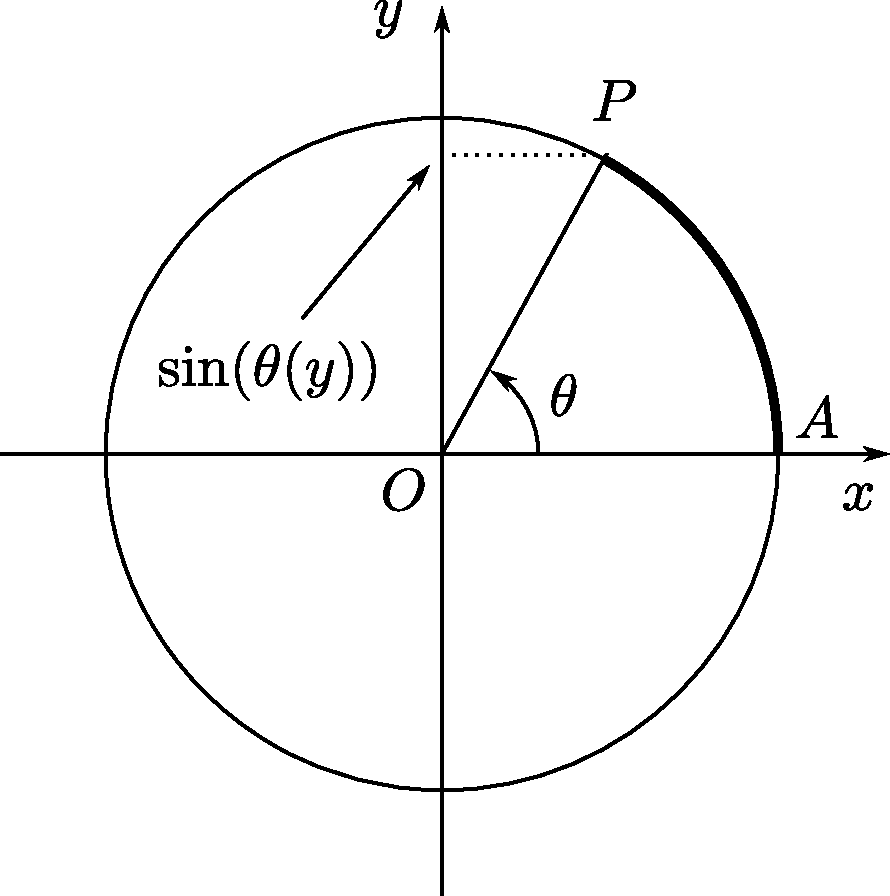
\includegraphics[width=60mm]{fig/circle.pdf}
    \subcaption{$P$が第1象限上の点の場合}
    \label{fig:circleposi}
  \end{minipage}
  \begin{minipage}{.45\linewidth}
    \centering
    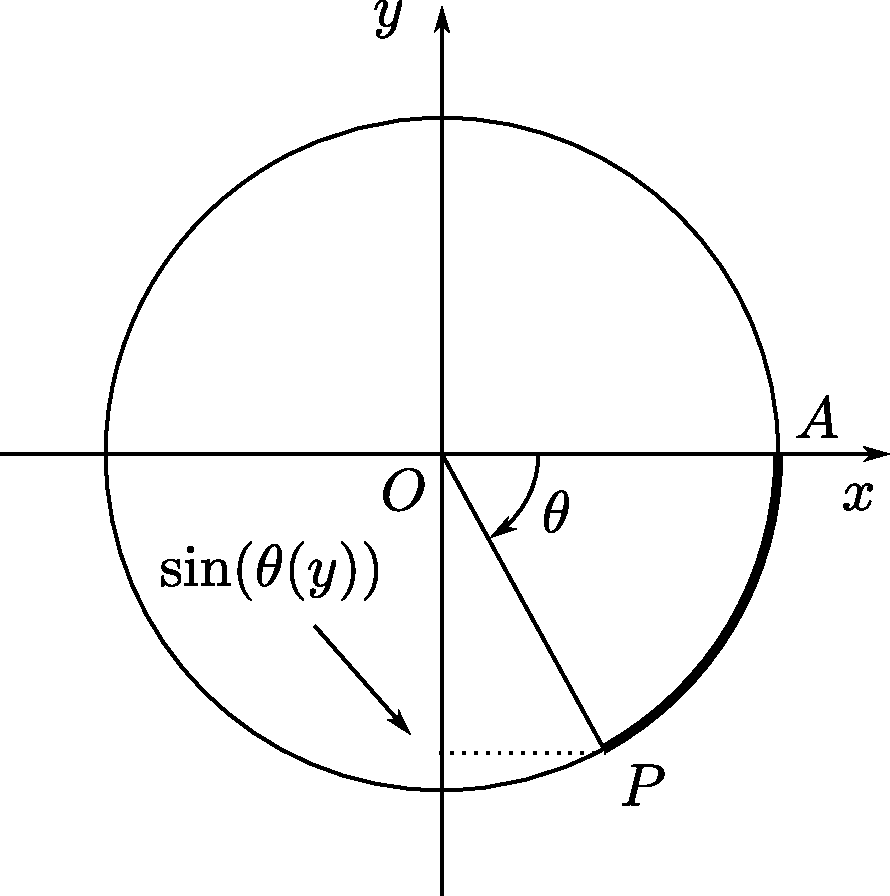
\includegraphics[width=60mm]{fig/circlenega.pdf}
    \subcaption{$P$が第4象限上の点の場合}
    \label{fig:circlenega}
  \end{minipage}
  \caption{$P$が第$1,4$象限上の点のときの\cref{dfn:sin}の幾何学的解釈,
    図の太線の部分の符号付き長さが$\apply{\theta}{y}$であり,$\apply{\sin}{\apply{\theta}{y}}$は$y$座標である.}
  \label{fig:circle}
\end{figure}

$P$が第2,3象限上の点である場合を考えよう.$P$が第2象限上の点,もしくは点$\coord{-1,0}$であるとする.
このとき,弧$AP$の長さは,上の関数$\theta$を用いれば,
$-1 < y < 0$であるような実数$y$を用いて$\apply{\theta}{y} + \pi$と表せる.このとき,
$P$の$y$座標は$-y$であるから,$P$の$y$座標は$- \apply{\sin}{\apply{\theta}{y}}$ということになる.
これは\cref{eq:sinperiod}より$\apply{\sin}{\apply{\theta}{y} + \pi}$と等しく,
やはり$P$の$y$座標は弧$AP$の符号付き長さに対応する$\sin$の値である.
$P$が第3象限上の点である場合にも同様に,弧$AP$の符号付き長さは$0 < y < 1$なる実数$y$を用いて
$\apply{\theta}{y} + \pi$と表せて,$P$の$y$座標は$- \apply{\sin}{\apply{\theta}{y}} = \apply{\sin}{\apply{\theta}{y} + \pi}$
だから,$P$の$y$座標は弧$AP$の符号付き長さに対応する$\sin$の値である.

\begin{figure}[htbp]
  \begin{minipage}{.45\linewidth}
    \centering
    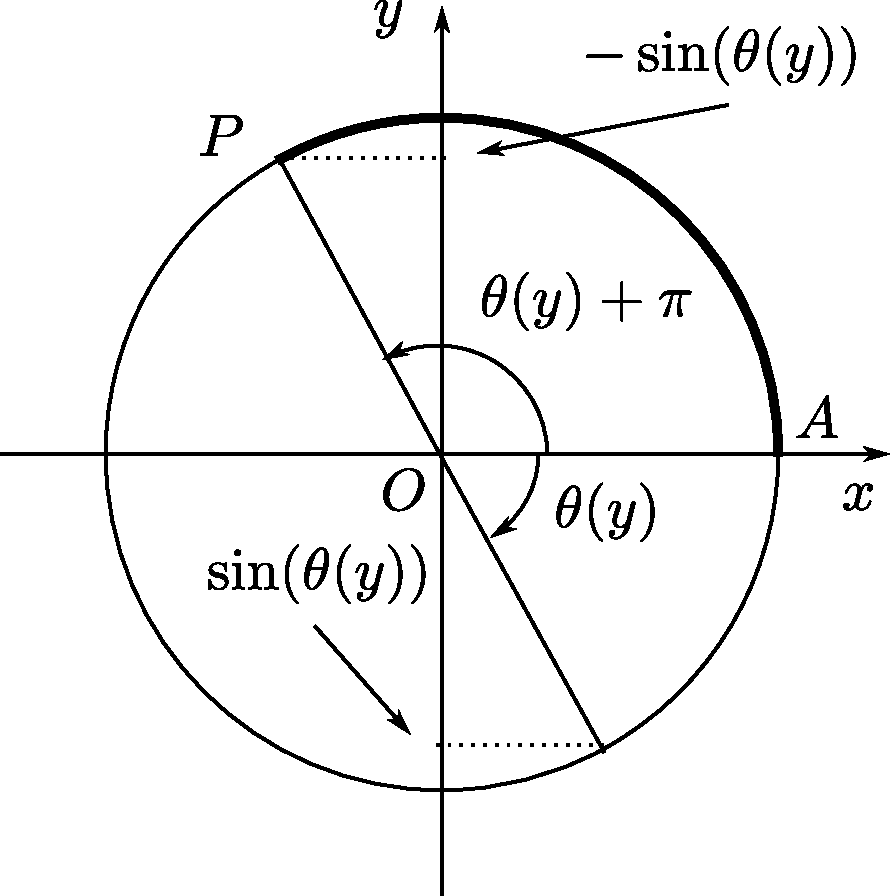
\includegraphics[width=60mm]{fig/circle2.pdf}
    \subcaption{$P$が第2象限上の点である場合}
    \label{fig:circle2}
  \end{minipage}
  \begin{minipage}{.45\linewidth}
    \centering
    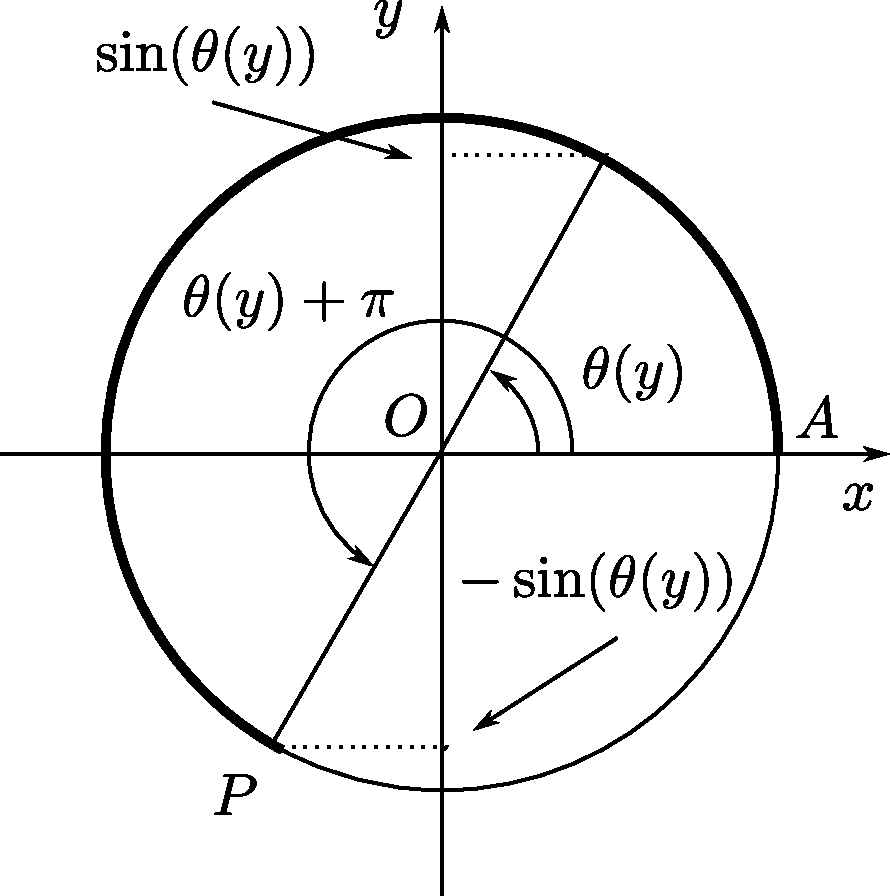
\includegraphics[width=60mm]{fig/circle3.pdf}
    \subcaption{$P$が第3象限上の点である場合}
    \label{fig:circle3}
  \end{minipage}
  \caption{$P$が第2,3象限上の点のときの\cref{dfn:sin}の幾何学的解釈,
    弧$AP$の符号付き長さは$\apply{\theta}{y} + \pi$であり,
    $P$の$y$座標は$\apply{\sin}{\apply{\theta}{y} + \pi} = - \apply{\sin}{\apply{\theta}{y}}$である.}
  \label{fig:circle23}
\end{figure}

以上で$-\frac{\pi}{2} \leq x < \frac{3\pi}{2}$を満たす実数$x$に関しては$\sin x$が高校の教科書に載っているものと
同じように解釈できることがわかった.他の場合については確かめてはいないが,\cref{lemma:period}から
どう解釈すればよいかはほとんど明らかであろうからいちいち解説するまでもないだろう.
なお,\cref{dfn:cos}で定義した関数$\cos$が高校の教科書に載っているものと同じものであることは同様にして確認できる.

\Cref{dfn:tan}に関して考えよう.$A = \coord{1,0}$とする.
実数$m$に対し,原点を中心とする半径1の円と直線$y = mx$との交点を$P$とすれば,
\cref{eq:arctanfunc}における$\apply{\theta}{m}$は弧$AP$の符号付き長さである.
関数$\tan$は,\cref{eq:arctanfunc}における関数$\theta$の逆関数であったから,
やはりこの関数$\tan$も高校の教科書に載っているものと同じものである.

\subsection{三角関数の基本性質} \label{subsec:identity}

三角関数が積分で定義された関数の逆関数として定義された以上,その導関数は\cref{thm:invderi}により簡単に計算できる.
まずはのちに使う公式を提示しておく.幾何学的に考察すればその成立はほとんど明らかであろう.

\begin{lemma} \label{lemma:sin2cos2}
  任意の実数$x$に対して
  \begin{align}
    \apply{\sin}{-x}    & = - \sin x,
    \label{eq:sinodd}                 \\
    \apply{\cos}{-x}    & = \cos x,
    \label{eq:coseven}                \\
    \sin^2 x + \cos^2 x & = 1
    \label{eq:sin2cos2}
  \end{align}
  が成り立つ.ただし,$\sin^2 x, \cos^2 x$はそれぞれ$\paren{\sin x}^2 ,\paren{\cos x}^2$の略記である.
  また,任意の$x \in \interval{op}{- \frac{\pi}{2}, \frac{\pi}{2}}$に対して
  \begin{align}
    \tan x = \frac{\sin x}{\cos x}
    \label{eq:tanfrac}
  \end{align}
  が成り立つ.さらに,これと\cref{eq:sin2cos2}から
  \begin{align}
    1 + \tan ^2 x = \frac{1}{\cos^2 x}
    \label{eq:tancos}
  \end{align}
  も得られる.
\end{lemma}

%\begin{proof}
%  幾何学的に考察すればこの主張が成り立つことはほとんど明らかである.
%  ここでは別の方法で証明してみよう.
%  \Cref{lemma:period}から$0 \leq x < 2\pi$の場合にのみ示せばよいことは明らかである.まずは$0 \leq x \leq \frac{\pi}{2}$のときに
%  \cref{eq:sin2cos2}が成り立つことを示そう.
%  $0 \leq x \leq \frac{\pi}{2}$を満たす任意の実数$x$に対し,
%  \begin{align*}
%    x = \bigintssss_0^{\sin x} \frac{\intd t}{\sqrt{1 - t^2}} = \bigintssss_{\cos x}^1 \frac{\intd t}{\sqrt{1 - t^2}}
%  \end{align*}
%  である.従って,
%  \begin{align*}
%      & \bigintssss_0^{\sin x} \frac{\intd t}{\sqrt{1 - t^2}} - \bigintssss_{\cos x}^1 \frac{\intd t}{\sqrt{1 - t^2}} \\
%      = & \bigintssss_0^{\sin x} \frac{\intd t}{\sqrt{1 - t^2}}
%      - \bigintssss_{\sqrt{1 - \cos^2 x}}^0 \frac{1}{u} \frac{-u}{\sqrt{1 - u^2}} \intd u \\
%      = & \bigintssss_0^{\sin x} \frac{\intd t}{\sqrt{1 - t^2}}
%      + \bigintssss_{\sqrt{1 - \cos^2 x}}^0 \frac{\intd t}{\sqrt{1 - t^2}} \\
%      = & \bigintssss_{\sqrt{1 - \cos^2 x}}^{\sin x} \frac{\intd t}{\sqrt{1 - t^2}} = 0 \text{.}
%  \end{align*}
%  ゆえに$\sin x = \sqrt{1 - \cos^2 x}$より\cref{eq:sin2cos2}を得る.
%
%  $\frac{\pi}{2} < x < \pi$とする.このとき,
%\end{proof}

\begin{thm} \label{thm:continus}
  $\sin, \cos, \tan$はいずれもそれぞれの定義域上の連続関数である.
\end{thm}

\begin{proof}
  $\sin$から考えよう.開区間$\interval{op}{-\frac{\pi}{2}, \frac{\pi}{2}}$上での
  連続性は微分積分学の基本定理から即座に従う.
  また,$\sin$が点$x$で連続ならば,任意の$n \in \Zahlen$に対して
  $\sin$は点$x + n\pi$でも連続である.これは\cref{eq:sinperiod}からわかる.
  従ってあとは2点$-\frac{\pi}{2}, \frac{\pi}{2}$での連続性のみを調べればよいが,
  これはすぐにわかる.$\cos, \tan$も同様である.
\end{proof}

\begin{thm} \label{thm:trigoderiv}
  関数$\sin, \cos, \tan$はその定義域上全域で微分可能であって,定義域上の各$x$に対して
  \begin{align}
    \diff*{\sin x}x & = \cos x,
    \label{eq:sinderiv}                    \\
    \diff*{\cos x}x & = - \sin x,
    \label{eq:cosderiv}                    \\
    \diff*{\tan x}x & = \frac{1}{\cos^2 x}
    \label{eq:tanderiv}
  \end{align}
  が成り立つ.
\end{thm}

\begin{proof}
  $\sin$から示そう.\cref{lemma:period}より閉区間$\interval{c}{-\pi, \pi}$上で考えればよい.
  開区間$\interval{op}{-\frac{\pi}{2},\frac{\pi}{2}}$上での微分可能性と
  \cref{eq:sinderiv}の成立は\cref{thm:invderi}と\cref{eq:sin2cos2}からすぐにわかる.
  また,開区間$\interval{op}{-\pi, -\frac{\pi}{2}}, \interval{op}{\frac{\pi}{2}, \pi}$上での
  微分可能性と\cref{eq:sinderiv}の成立は,
  \cref{eq:sinperiod}を用いればよい.
  その他の点での微分可能性は\cref{thm:derivcont}による.
  $\cos$についても同様で,$\tan$に関しては\cref{eq:tanfrac}を用いればよい.
\end{proof}

\begin{coro} \label{coro:sinlim}
  \begin{align}
    \lim_{x \to 0} \frac{\sin x}{x} = 1 \text{.}
    \label{eq:sinlim}
  \end{align}
\end{coro}

\begin{proof}
  \Cref{eq:sinderiv}による.
\end{proof}

\begin{thm}[加法定理] \label{thm:trigosum}
  任意の実数$\alpha, \beta$に対して
  \begin{align}
    \apply{\sin}{\alpha + \beta} & = \sin \alpha \cos \beta + \cos \alpha \sin \beta,
    \label{eq:sinsum}                                                                 \\
    \apply{\cos}{\alpha + \beta} & = \cos \alpha \cos \beta - \sin \alpha \sin \beta
    \label{eq:cossum}
  \end{align}
  が成り立つ.また,$\alpha, \beta , \alpha + \beta$のいずれも$\frac{\pi}{2}$の整数倍にならないような
  実数$\alpha, \beta$に対して
  \begin{align}
    \apply{\tan}{\alpha + \beta} = \frac{\tan \alpha + \tan \beta}{1 - \tan \alpha \tan \beta}
    \label{eq:tansum}
  \end{align}
  が成り立つ.
\end{thm}

\begin{proof}
  三角関数の周期性や相互関係をうまく使って特殊な場合に帰着させ,
  座標平面上に三角形を埋め込んで幾何学的に考察してもよいが,
  \cref{thm:trigoderiv}を使えばもっと簡単に示すことができる.
  任意の実数$x, \beta$に対し,行列に関して
  \begin{align}
    \begin{bmatrix}
      \cos x   & \sin x \\
      - \sin x & \cos x \\
    \end{bmatrix}
    \begin{bmatrix}
      \apply{\cos}{x + \beta} \\
      \apply{\sin}{x + \beta} \\
    \end{bmatrix}
    =
    \begin{bmatrix}
      \cos x \apply{\cos}{x + \beta} + \sin x \apply{\sin}{x + \beta}   \\
      - \sin x \apply{\cos}{x + \beta} + \cos x \apply{\sin}{x + \beta} \\
    \end{bmatrix}
    \label{eq:rotationinv}
  \end{align}
  が成り立ち,この式の右辺の1行目と2行目をそれぞれ$\apply{f}{x}, \apply{g}{x}$として
  関数$f,g \colon \Real \to \Real$を定義すれば,$f,g$は$\Real$上で微分可能であって,
  その導関数はともに恒等的に0となる.従って$f,g$は定数関数で,\cref{eq:rotationinv}は
  \begin{align}
    \begin{bmatrix}
      \cos x   & \sin x \\
      - \sin x & \cos x \\
    \end{bmatrix}
    \begin{bmatrix}
      \apply{\cos}{x + \beta} \\
      \apply{\sin}{x + \beta} \\
    \end{bmatrix}
    =
    \begin{bmatrix}
      \cos \beta \\
      \sin \beta \\
    \end{bmatrix}
    \label{eq:rotationinvbeta}
  \end{align}
  と書き換えられる.この式の両辺に行列
  \begin{align*}
    \begin{bmatrix}
      \cos x & - \sin x \\
      \sin x & \cos x   \\
    \end{bmatrix}
  \end{align*}
  を左からかけて
  \begin{align}
    \begin{bmatrix}
      \apply{\cos}{x + \beta} \\
      \apply{\sin}{x + \beta} \\
    \end{bmatrix}
    =
    \begin{bmatrix}
      \cos x \cos \beta - \sin x \sin \beta \\
      \sin x \cos \beta + \cos x \sin \beta \\
    \end{bmatrix}
    \label{eq:trigosumx}
  \end{align}
  が得られ,$x = \alpha$を代入して\cref{eq:sinsum,eq:cossum}が得られる.
  \cref{eq:tansum}は\cref{eq:sinsum,eq:cossum}と\cref{eq:tanfrac}から得られる.
\end{proof}

\section{高校の教科書における三角関数論の正当性} \label{sec:highschool}

先の議論で展開した三角関数論は,定義までは高校の教科書に載っているものを精密化したものであったが,
その後の議論は高校の教科書とは大きく異なっていた.
これに関連して,「高校の教科書における三角関数の微分公式の導出は循環論法だ」
という主張がなされることがある.
その主張は,高校の教科書では\cref{coro:sinlim}から\cref{thm:trigosum}を経て\cref{thm:trigoderiv}を示すのだが,
その\cref{coro:sinlim}を証明する際に用いられる扇形の面積公式の導出に
\cref{thm:trigoderiv}(から導かれる三角関数の積分公式)が用いられているというものである.
しかし,扇形の面積公式は\cref{thm:trigoderiv}によらずに示すことができる.

\Cref{fig:sector}のように,原点を中心とする半径1の円の第1象限の部分に点$P = \coord{x,y}$をとり,
$A = \coord{1,0}$とする.
弧$AP$の長さは\cref{eq:theta}における関数$\theta$を用いて$\apply{\theta}{y}$と表される.
このとき,扇形$OAP$の面積$S$は
\begin{align*}
  S & = \int_0^y \sqrt{1 - x^2} \intd x - \frac{xy}{2}                                                                                            \\
    & = y \sqrt{1 - y^2} - \bigintssss_0^y \frac{1 - t^2}{\sqrt{1 - t^2}} \intd t + \bigintssss_0^y \frac{\intd t}{\sqrt{1 - t^2}} - \frac{xy}{2} \\
    & = \apply{\theta}{y} - \paren{ \int_0^y \sqrt{1 - t^2} \intd t - \frac{xy}{2}}                                                               \\
    & = \apply{\theta}{y} - S
\end{align*}
と計算できるから,
\begin{align}
  S = \frac{1}{2} \apply{\theta}{y}
\end{align}
となって扇形の面積公式が導かれる.

\begin{figure}[htbp]
  \centering
  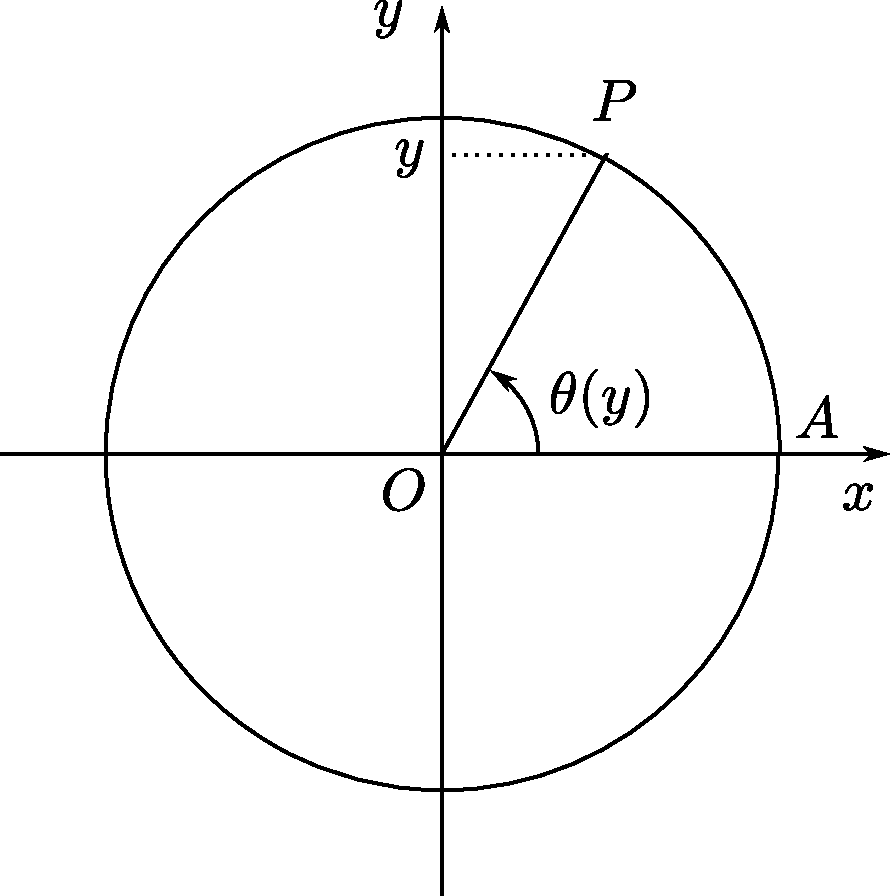
\includegraphics[width=70mm]{fig/sector.pdf}
  \caption{扇形の面積公式の証明,図の点線の長さは$\sqrt{1 - y^2}$である.}
  \label{fig:sector}
\end{figure}




\end{document}
